%
% Template for Department of Electrical and Information Engineering Diploma Thesis v1.1.2013
% Authors: Mika Korhonen (original author), Pekka Pietikäinen, Christian Wieser, Teemu Tokola and Juha Kylmänen.
% If you make any improvements to this template, please contact ouspg@ee.oulu.fi
%

\documentclass[a4paper,12pt,titlepage]{dithesis}
\usepackage[english,finnish]{babel}
\usepackage[utf8]{inputenc}
\usepackage[T1]{fontenc}
\usepackage{times}
\usepackage{tabularx}
\usepackage{graphicx}
\usepackage{float}
\usepackage{enumerate}
\usepackage{placeins}
\usepackage{fancybox}
\usepackage{verbatim}
\usepackage{longtable}
\usepackage{di}
\usepackage[hyphens]{url}
\usepackage{boxedminipage}
\usepackage{subfigure}
\usepackage{multirow}
% my additions
\usepackage{listings}
\usepackage{alltt}
\usepackage{changepage}   % for the adjustwidth environment
% For screenshots, etc.
\usepackage{graphicx}
\graphicspath{ {images/} }
% end of additions
\tolerance=500

%\usepackage[a4paper,margin=2.5cm,dvips]{geometry}
%\geometry{papersize={210mm,297mm}}
%dvipdf -sPAPERSIZE=a4

% The following code removes %-signs with URL:s longer than 72 chars
\begingroup
\makeatletter
\g@addto@macro{\UrlSpecials}{%
  \endlinechar=13 \catcode\endlinechar=12
  \do\%{\Url@percent}\do\^^M{\break}}
 \catcode13=12 %
 \gdef\Url@percent{\@ifnextchar^^M{\@gobble}{\mathbin{\mathchar`\%}}}%
\endgroup %

%\selectlanguage{finnish}


\otsikko{Turvallinen käyttöönotto haastavissa ympäristöissä}
\title{Secure Deployment Story for Challenging Environments}

\etunimi{Ossi}
\sukunimi{Herrala}
\valvoja{prof. Juha Röning}
\koulutusohjelma{electrical} % {information | electrical}
\vuosi{2017}
\tyo{Bachelor} % {Bachelor | Master}
\kieli{english} % {finnish | english}

\begin{document}

\begin{titlepage}
	%\vspace*{10 mm}
	\centering{\includegraphics*[width=0.5\textwidth]{uni_logo}\\}
	{{\small FACULTY OF INFORMATION TECHNOLOGY AND ELECTRICAL ENGINEERING}\\}
	\vspace{65 mm}
	{\textbf{\LARGE \getfirstname\ \getlastname}\\}
	\vspace{15 mm}
	{\textbf{\LARGE SECURE DEPLOYMENT STORY\\FOR CHALLENGING ENVIRONMENTS\\}}
	\vspace{70 mm}
	{\large {Bachelor's Thesis}\\}
	{\large {Degree Programme in Electrical Engineering}\\}
	{\large {April 2017}\\}
	%\maketitle
\end{titlepage}

\selectlanguage{english}

\begin{abstract}

\iffalse
\begin{itemize}
\item FIXME: remove this list
\item Background information (present tense)
\item Principal activity (past tense/present perfect tense)
\item Methodology (past tense)
\item Results (past tense)
\item Conclusions (present tense/tentative verbs/modal auxiliaries)
\end{itemize}
\fi

Network based automatic installation of an operating system is and has
been a crucial method to manage masses of computers. Protecting every
step of the installation is important. Ability to trust the
installation system to complete operating system installation safely
and produce secure installation is important step in information
security life cycle.

This thesis reviews past and current state of network based automatic
installation systems based on what protocols do they use. Then it
continues to identify risks to those protocols and study how the
situation could be improved by using cryptography using Transport
Layer Security (TLS) protocol and digital signatures. This thesis
shows how these two existing technologies can be used to provide more
secure installation system.

Proof of concept implementation using TLS and digital signatures is
specified, developed and then compared to already existing and
publicly available installation system.

\keywords deployment, network protocol, operating system, installation system, network security
\end{abstract}

\selectlanguage{finnish}
\begin{tiivistelma}

Automaattinen käyttöjärjestelmän asennus verkon yli on ollut ja on
edelleen tärkeä tapa hallita isoja määriä tietokoneita. Jokaisen
asennusvaiheen suojaaminen on tärkeää. Mahdollisuus luottaa
asennusjärjestelmän toimivan turvallisesti ja tuottavan turvallisen
asennuksen on tärkeää tietoturvan elinkaaressa.

Tämä kandidaatintyö käy läpi miten asennusjärjestelmät ovat toimineet
ennen ja nykyisin sen perusteella mitä protokollia ne
käyttävät. Seuraavaksi tunnistetaan prokotolliin liittyviä riskejä ja
miten tilannetta voisi parantaa käyttämällä salausta (Transport Layer
Security, TLS) ja digitaalisia allekirjoituksia. Kandidaatintyö
osoittaa, että näitä kahta olemassaolevaa teknologiaa voi käyttää
tuottamaan turvallisemman asennusympäristön.

Asennusjärjestelmästä määriteltiin ja toteutettiin soveltuvuusselvitys
hyödyntäen TLS teknologiaa ja digitaalisia allekirjoituksia. Tätä
järjestelmää verrattiin julkisesti saatavilla olevaan
asennusjärjestelmään.

\avainsanat käyttöönotto, verkkoprotokolla, käyttöjärjestelmä, asennusjärjestelmä, verkon tietoturva
\end{tiivistelma}

\selectlanguage{english}
%\selectlanguage{finnish}

\sisluettelo
%\tableofcontents

\otsake{FOREWORD}

\iffalse
Your personal background (in brief)
Your personal experiences or the circumstances that motivated you to write your dissertation (in brief)
The target group for which your dissertation was written
The division of labor (when the dissertation has been written by more than one person)
Acknowledgements to individuals and institutions who have helped you in the writing and checking of the dissertation
\fi

I have been writing software, and designing, building, operating and
tearing down Linux and UNIX systems for two decades. Installing
operating system has been important part of life cycle of Linux and
UNIX systems.

This thesis was motivated by the need for modernizing operating system
installation over Internet. It is big subject with lots of little
details to work on. This thesis is just small but important part of
it.

I hope my work with this thesis can contribute back to everyone who
has made my life so much easier with their installation systems.

I would like to thank my supervisor Prof. Juha Röning for the
opportunity to do this thesis for Oulu University Secure Programming
Group. Huge thanks to Christian Wieser for continuously taking the
time to sit down with me for followup and pushing me forward.

Thanks to everyone who attended OUSPG Open
2016\footnote{https://github.com/ouspg/ouspg-open} and especially for
everyone who participated the Thesis Review session, and read my work
and gave feedback. Truly appreciated.

Thanks to my dad and sister for taking the time to read my work and
giving valuable feedback. Hugs to my spouse Ella, who not only read
and commented my work, but also endured the process of me writing it
while also finishing her master's degree.


%\allekirjoitus{Oulu, Finland \today}

\otsake{ABBREVIATIONS}

\setlongtables
\begin{longtable}[l]{p{3cm}p{0.7\textwidth}}
  % Add your abbreviations to abbreviations.tex
  BOOTP  & Bootstrap Protocol (IETF)                     \\
CIA    & Confidentiality, Integrity, Availability      \\
DHCP   & Dynamic Host Configuration Protocol (IETF)    \\
DNS    & Domain Name System (IETF)                     \\
DNSSEC & Domain Name System Security Extensions (IETF) \\
FTP    & File Transfer Protocol (IETF)                 \\
GPG    & The GNU Privacy Guard                         \\
HTTP   & Hypertext Transfer Protocol (IETF)            \\
HTTPS  & HTTP over TLS                                 \\
IETF   & Internet Engineering Task Force               \\
IP     & Internet protocol (IETF)                      \\
IPMI   & Intelligent Platform Management Interface     \\
MitM   & Man-in-the-Middle                             \\
NFS    & Network File System (IETF)                    \\
NSA    & National Security Agency                      \\
PXE    & Preboot Execution Environment                 \\
RARP   & A Reverse Address Resolution Protocol (IETF)  \\
RFC    & Request for Comments (IETF)                   \\
RSA    & Public-key cryptosystem named after Ron Rivest, Adi Shamir and Leonard Adleman \\
TFTP   & Trivial File Transfer Protocol (IETF)         \\
TLS    & Transport Layer Security (IETF)               \\
UDP    & User Datagram Protocol (IETF)                 \\
URL    & Uniform Resource Locator                      \\
USB    & Universal Serial Bus                          \\
USENIX & The Advanced Computing Systems Association    \\
initrd & initial ramdisk                               \\

\end{longtable}
\setcounter{table}{0}

%Johdanto
\chapter{Introduction}
\sivunumerot{}
% Introduction Chapter

\begin{itemize}
\item INTRODUCTION: The Setting - bird eye's view - the challenge to be tackled / thing to be be improved in general
\item INTRODUCTION: Past research done
\item INTRODUCTION: Gap in knowledge/problem not yet solved
\item INTRODUCTION: Purpose and method of this work
\item INTRODUCTION: More detailed description what was done
\item INTRODUCTION: Results acquired
\item INTRODUCTION: Analysis and limitations of the result (Mostly relocate to Conclusions)
\item INTRODUCTION: Value (Mostly relocate to Conclusions)
\end{itemize}

Lorem ipsum dolor sit amet, consectetur adipiscing elit. Pellentesque lobortis eget dolor nec vehicula.
Donec pretium dui at bibendum accumsan \cite{cheswick}. Aliquam sollicitudin pharetra felis, in euismod velit volutpat 
vitae. Praesent iaculis id est sed ultrices. Nunc pretium euismod dolor, nec molestie elit ultricies a. 
Praesent laoreet mi metus, eu luctus dui lobortis vel. Vivamus sit amet elementum augue, ac lacinia leo.

Aenean vel est pellentesque, malesuada dolor nec, porta diam. Quisque molestie quis nibh quis facilisis. 
Nam placerat, ante imperdiet adipiscing rhoncus, quam augue consequat ligula, eu porttitor velit turpis 
a sem. Donec nibh dolor, sagittis in metus at, porta lacinia risus. Vestibulum quis rhoncus massa, eu 
eleifend metus. Curabitur vehicula malesuada enim at rutrum. Praesent eu velit porta, lacinia tortor ac, 
fermentum libero. \cite{kamara, al-shaer}


\section{Sample section with a table reference}

Ut hendrerit volutpat felis vitae aliquam. Duis quis augue urna. In sollicitudin lacinia elit, 
non ultrices dui tristique eu. In hac habitasse platea dictumst. Nullam mi sapien, sagittis non 
mi in, gravida lobortis ante. A sample latex table can be seen in Table~\ref{tab:sample_table}.


\begin{table}[!ht]
% Add some padding to the table cells:
\def\arraystretch{1.1}%
\begin{center}
  \caption{Sample table}
  \label{tab:sample_table}
  \begin{tabular}{| l | c | }
    \hline
    Sample & table \\
    \hline
    Sample & table \\
    Sample & table \\
    \hline
  \end{tabular}

  \end{center}
\end{table}

\section{Changelog}

\begin{itemize}
\item Changed \textit{\textbackslash{chapter's}} \textbackslash{newpage} to 
\textbackslash{clearpage} to prevent floats from wandering to the beginning of the next chapter

\item Added \textbf{[hyphens]} to the url package to prevent margin overflow with 
long urls

\item Added \textbf{multirow} package to make multirow and multicolumns possible

\item Added some helpful source code comments

\item Makefile for pdflatex and bibtex to automate pdf compilation

\item Abbreviations are autosorted by the Makefile

\item Added a bit of extra padding to the sample table
\end{itemize}

\subsection{Sample subsection with a figure reference}

Sed erat neque, cursus ac feugiat ac, sollicitudin
ut odio. Maecenas vel turpis rhoncus, euismod nisl ac, tincidunt ipsum. Curabitur fermentum vel
turpis ac lobortis. Cras a justo vitae diam volutpat blandit. Maecenas faucibus nibh a neque 
semper ullamcorper. Suspendisse in est vulputate, fermentum odio nec, pharetra augue. Fusce at
consequat arcu, sed hendrerit enim. Pellentesque id suscipit nibh, id pretium erat. 

Nam eget libero neque. Nullam commodo cursus turpis mollis cursus. Curabitur est tellus,
pellentesque eu velit sed, ullamcorper gravida felis. Proin vel cursus risus, at scelerisque 
justo. Quisque rutrum justo at ultricies auctor. A sample latex figure can be seen in
Figure~\ref{fig:oylogoe}. If your pictures appear grainy, you probably have too low dots
per inch (DPI) value.

\footnotetext[1]{Sample footnote}

%Pictures in .eps if you use latex, .pdf or .png if you use pdflatex. Don't specify the extension so you can use both!
\begin{figure}[ht]
  \begin{center}
    \includegraphics*[width=0.3\textwidth]{oylogoe}
  \end{center}
  \caption{A picture}
  \label{fig:oylogoe}
\end{figure}

 % ./introduction.tex

\chapter{Implementing secudep}
% Implementation Chapter

To see if it's possible to use HTTPS and digital signatures, a simple
proof of concept implementation of installation system
called \emph{secudep} was implemented. Source code can be found from
secudep's project site on
GitHub~\footnote{https://github.com/ouspg/secudep}.

Secudep's implementation has three main design principles: ease of
use, ease of deploy and security. Deploying new installation system
should be easy so that it encourages building small, easy to update
and easy to maintain setups. Ease of deployment might also attract
developing new use cases and applications on top of already existing
system. With the implemented solution there should be no need to have
monolithic and centralized installation system, but designs can shift
more towards personal or per application installation systems.

Installation system should help end user achieve fresh installation of
operating system and applications as easily, smoothly and as fast as
possible. Most of the decisions required for achieving installation
should be made beforehand and automatized as much as feasible.

Security is more difficult design principle to tackle. For the
installation system the concentration should be on selecting and
enforcing safe defaults, and guide user to make safe choices.

The proof of concept implementation uses public-key cryptography to
digitally sign files so that the authenticity of those files can be
verified. It should also be encouraged to regenerate new key material
when updating signature files. This renders old installation system
unusable and forces updating of installation media (for example USB
mass media).

One security design principle is, for example, to halt the
installation process when a security measure detects an anomaly. Such
anomaly could for example be an active Man in the Middle attack. If
user is given a choice to continue, she usually does so. Probably
without understanding or investigating what caused the issue, thus
rendering the security measure useless and allowing the attack.

This implementation borrows lots of ideas and lessons learned from
boot.foo.sh~\cite{boot-foo-sh} and from installation system
used by Faculty of Information Technology and Electrical Engineering
in University of Oulu.

\section{Tools}

Secudep uses iPXE~\cite{iPXE} as a network boot firmware.\@ iPXE is a
PXE~\cite{PXEspec} implementation with additional features such as
support for booting via HTTP~\cite{RFC2616} protocol. Support for
HTTPS can also be compiled in.\@

Secudep's iPXE binary build is done inside container using
Docker~\cite{Docker} software containerization platform to achieve
repeatable builds with managed dependencies. Docker is tool to easily
build operating system level virtualization~\cite{Soltesz2007}
containers. Instead of virtualizing the hardware like Xen or KVM,
containers use operating system's namespaces to separate containerized
applications from each other. Docker is not mandatory for producing
the build.

Python programming language, bash shell scripts and OpenSSL are used
to build individual parts of the system.

\section{Setting up installation system}

Setting up the installation system using secudep has the following
steps. After the list, all the steps are explained further.

\begin{enumerate}
  \item Generate digital signing keys
  \item Collect HTTPS servers' X.509 certificates for public key pinning
  \item Build iPXE bootable media
  \item Write configuration file
  \item Generate contents for deployment
\end{enumerate}

Digital signing keys are generated when deploying the installation
system. Private key is used to produce the signatures and
public key is embedded into the installation image.

The installation system is deployed to known HTTPS server. Thus this
server's X.509 certificate can be fetched and embedded into
installation image. This is now the only X.509 certificate to be
trusted and no other HTTPS server can be used.

When digital signing keys are generated and X.509 certificates are
fetched, it's possible to build the bootable installation media. This
installation media file is written for example to USB memory and can
be used to launch the operating system installation in a computer.

Configuration file binds things together. It specifies the HTTPS
server, where the keys and certificates are and what operating systems
can be installed and where the required files can be found.

After all other steps are done, the files to be deployed on HTTPS
server can be generated. This step fetches all required files,
calculates digital signatures and various boot scripts, and builds
directory structure which then should be mirrored on the HTTP server.

Future work on secudep should simplify these steps even further.
Digital signing keys could be automatically generated if missing,
X.509 certificate collection could be automated based on secudep's
configuration file.\@ iPXE media build could also be done every time
contents for deployment are generated.

\section{Deploying}

Everything needed for installation system to operate (from server
side) are generated under one directory. This directory can then be
published on HTTPS server. The URL for the installation system files
is configured in secudep's configuration file.

\section{Security}

Secudep make it as easy as possible to use public key pinning for
HTTPS hosts and digital signatures to verify authenticity of files.

iPXE is configured to require trusted files. File is trusted only
after it's signature is verified successfully. This requirement can't
be turned off once it's turned on.
  % ./implementation.tex

\chapter{Case studies}
% Testing Chapter

%% FIXME: Case study 1 (What, how, )

%%  * Describe test setup
%%  * For each case study - test case
%%  * Experiment -
%%    * clearly described test aim (What?)
%%    * How / What are the specifics of this test case / case study?
%%    * RESULTS
%%    * ANALYSIS


\section{Case Study 1: Identify Protocols}
\label{sec:casestudy1}

\subsection{What was studied}

The purpose of this case study is to identify network protocols used
in online installation infrastructure system. This study also verifies
the involved protocols which were described in the introduction
chapter.

For installation infrastructure a service called
boot.foo.sh~\cite{boot-foo-sh} is used. Boot.foo.sh was chosen because
it's open service known to be used to automatic installations in
enterprises and it has been an inspiration to this thesis to make
installation infrastructure more safer to use.

Boot.foo.sh is used to install CentOS~7 Linux operating system. CentOS
Linux is community driven effort to provide free alternative to Red
Hat Enterprise Linux (RHEL). CentOS is built using RHEL source
code. Red Hat has 67 \% market share of Linux distribution market
according to Gartner's analysis~\cite{gartner-redhat}.

\subsection{How it was done}

The installation was done using virtual machine. VirtualBox was chosen
as a virtualization software because it's free, open source and has
easy to use network traffic recording functionality.

\begin{figure}[h]
  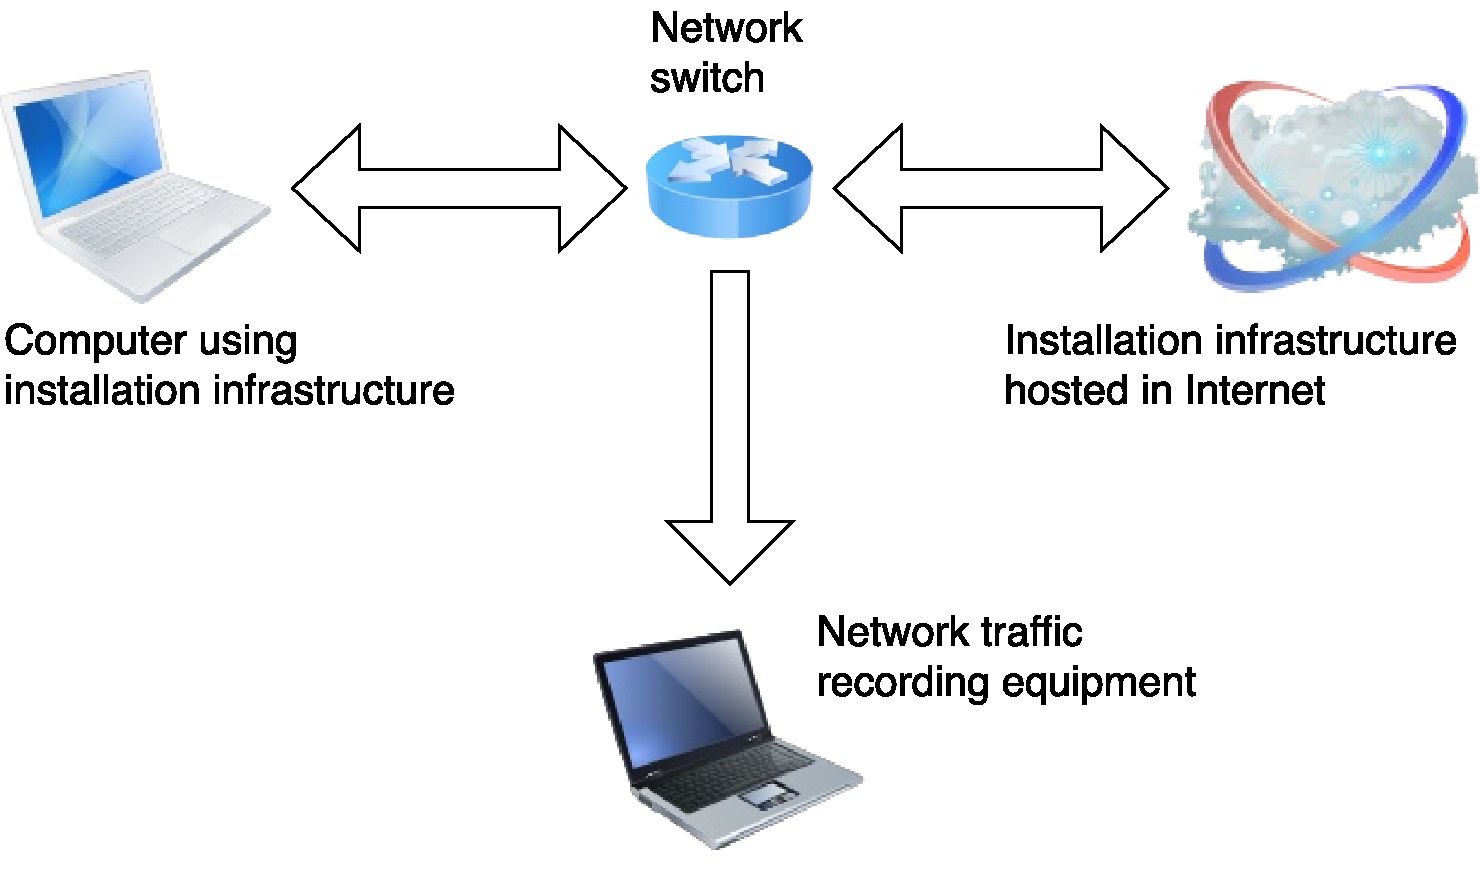
\includegraphics[width=\textwidth]{network-recording.pdf}
  \caption{Network traffic recording setup.\label{fig:network-recording}}
\end{figure}

With VirtualBox's network traffic recording it's possible to get
network traffic captured for the whole lifetime of virtual
machine. The capture is saved as standard PCAP file which can later be
opened in network protocol analyzer for
investigation. Figure~\ref{fig:network-recording} has the typical
traffic capturing setup with computer using the installation
infrastructure, another computer recording the traffic, network switch
to arrange traffic flows and the Internet containing the installation
infrastructure in use.

Traffic capture was then analyzed using Wireshark network protocol
analyzer. Wireshark is free and open source network protocol analyzer
which has capability to help expert user analyze many different
network protocols and their internals.

Traffic analysis was done by hand looking the captured traffic
recording and identifying protocols used.

\subsection{Results found}

Traffic recording was 788 megabytes of network traffic containing over
883 thousand network packets. Recording contains time span of a bit
over nine minutes.

\begin{table}[!ht]
  % Add some padding to the table cells:
  \def\arraystretch{1.1}%
  \begin{center}
    \begin{tabular}{| l | l |}
      \hline
      Step               & protocol    \\
      \hline
      Address resolution & DHCP        \\
      Name resolution    & DNS         \\
      Boot menu          & HTTPS       \\
      kernel and initrd  & HTTP        \\
      Kickstart          & HTTP        \\
      Installation files & HTTP (DS)   \\
      \hline
    \end{tabular}
    \caption{Table of found protocols and their role. DS in table
      means Digital Signatures.\label{tab:found_protocols_table}}
  \end{center}
\end{table}

Summary of the protocols used in various steps of installation process
can be found from Table~\ref{tab:found_protocols_table}.

Steps are identified and named for each system used to achieve the
installation. The steps are discussed in chronological order of
appearance as found from traffic recording.

\subsection{Analysis of results}

``Address resolution'' is the first step and it's purpose is to get IP
address and DNS server addresses for system to be installed. DHCP is
the standard protocol for this, and was also found to be used here.

``Name resolution'' is used to translate host names into IP address to
communicate with other servers. DNS protocol is used for name
resolution needs.

\begin{figure}[h]
  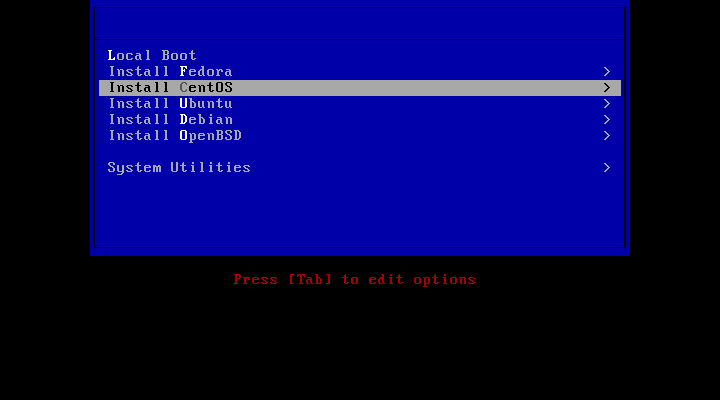
\includegraphics[width=\textwidth]{bootfoosh-bootmenu.png}
  \caption{boot.foo.sh boot menu showing selection of operating
    systems.\label{fig:bootmenu}}
\end{figure}

``Boot menu'' is used to display choices of operating systems to be
installed. Boot menu from boot.foo.sh can be seen in
figure~\ref{fig:bootmenu}. Boot.foo.sh uses HTTP protocol to fetch
various files needed to display the boot menu.

``kernel and initrd'' are the files needed to launch Linux
installation. These two files are downloaded over the Internet and
then kernel is executed and it continues the boot process. HTTP was
used to communicate with CentOS 7 mirror to fetch the needed files.

``Kickstart'' is CentOS specific file for automating unattended
installation. It's set of instructions downloaded and executed by the
installation process. Kickstart file is downloaded by software inside
initrd system so at this point the control of installation is already
switched to CentOS' installer. HTTP was used to communicate with
boot.foo.sh server to fetch the kickstart file.

``Installation files'' are the contents of operating system to be
installed. The files are downloaded and extracted to hard drive to
achieve the installation. Operating system installer is usually
trusted to verify digital signatures (e.g. CentOS uses
OpenPGP~\cite{RFC4880} (``GPG'') signatures) the downloaded content
before extracting the files into hard drive. The CentOS
documentation~\cite{centos-gpg} states that

\begin{quote}
Each stable RPM package that is published by CentOS Project is signed
with a GPG signature. By default, yum and the graphical update tools
will verify these signatures and refuse to install any packages that
are not signed, or have an incorrect signature. You should always
verify the signature of a package prior to installation. These
signatures ensure that the packages you install are what was produced
by the CentOS Project and have not been altered by any mirror or
web site providing the packages.
\end{quote}

However, when initrd file is downloaded over insecure protocol or file
content is not verified against signature it's possible for malicious
third party to inject it's own OpenPGP keys into initrd and point
installation system to malicious host serving the operating system
installation files and thus gain full control of the installed system.


\section{Case Study 2: Comparing boot.foo.sh and secudep}
\label{sec:casestudy2}

\subsection{What was studied}

Compare results from case study 1 to how secudep works.

\subsection{How it was done}



\subsection{Results found}

\begin{table}[!ht]
  % Add some padding to the table cells:
  \def\arraystretch{1.1}%
  \begin{center}
    \begin{tabular}{| l | l | l |}
      \hline
      Step               & boot.foo.sh   & secudep    \\
      \hline
      Address resolution & DHCP          & DHCP       \\
      Name resolution    & DNS           & DNS        \\
      Boot menu          & HTTP          & HTTPS (DS) \\
      Digital signatures & N/A           & HTTPS      \\
      kernel and initrd  & HTTP          & HTTP (DS)  \\
      Kickstart          & HTTP          & HTTPS      \\
      Installation files & HTTP (DS)     & HTTP (DS)  \\
      \hline
    \end{tabular}
    \caption{Comparison between how boot.foo.sh and secudep use of
      protocols. DS in table means Digital
      Signatures.\label{tab:comparison_table}}
  \end{center}
\end{table}

Results of comparing boot.foo.sh and secudep can be found from
Table~\ref{tab:comparison_table}. Boot.foo.sh results are same as in
case study 1.

The differences between boot.foo.sh and secudep in
Table~\ref{tab:comparison_table} are discussed next.

''Boot menu'' is used to display choices of operating systems to be
installed. HTTP is used in boot.foo.sh. HTTP protocol is susceptible
to Man in the Middle attack. Secudep uses HTTPS (HTTP over TLS) with
signed files to redemiate this issue.

\begin{figure}[h]
  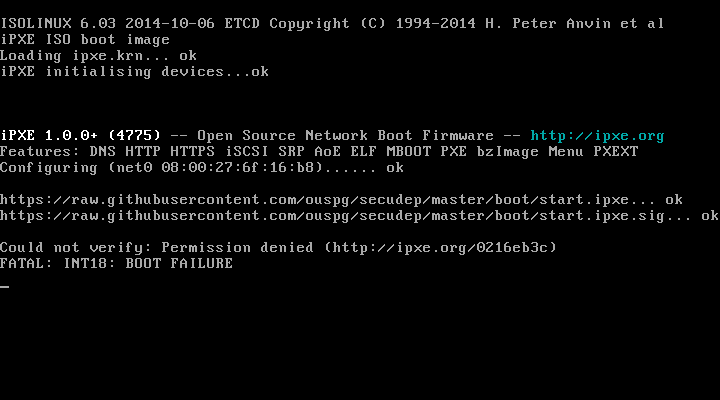
\includegraphics[width=\textwidth]{verify-fail.png}
  \caption{Installation process is halted when digital signature
    verification fails.\label{fig:verify-fail}}
\end{figure}

Only secudep uses digital signatures and the signature files are
fetched over HTTPS.\@ This is a step missing from
boot.foo.sh. Figure~\ref{fig:verify-fail} shows how secudep's process
is halted when the digital signature verification fails. This failure
is a clear indication that something is wrong.

Kernel and initrd are the files needed to launch the Linux
installation. Both boot.foo.sh and secudep systems use HTTP
protocol. Again HTTP is susceptible to Man in the Middle attacks. HTTP
is used because the files are fetched from CentOS's official mirror
over the internet. Secudep uses digital signatures to verify
downloaded content. After kernel and initrd are downloaded and digital
signatures are verified the execution is handled to kernel. This means
that secudep can't provide digital signatures to any following files.
  % ./testing.tex

% \chapter{Discussion and conclusion}
% % Conclusions and discussion Chapter

\begin{itemize}
\item CONCLUSIONS: reference to purpose of study
\item CONCLUSIONS: value of / reasons for the study
\item CONCLUSIONS: review of important findings / conclusions
\item CONCLUSIONS: comments, explanations or speculations about findings
\item CONCLUSIONS: limitations of study
\item CONCLUSIONS: implications of study or generalizations
\item CONCLUSIONS: recommendations for future or practical applications - USUALLY SKIPPED
\end{itemize}

This thesis took a look what network based threats could face
installation infrastructure and then studied what kind of means could
be used to protect the initial phases (before OS kernel took the
control of excecution) of installation process using encryption and
file signing.

Protecting every step of communications over networks is important and
protecting installation infrastructure is no exception. This thesis
has shown that it's possible to take a step further in a more secure
installation infrastructure by using two technologies: encryption and
file signatures.

More secure systems can be build step by step by combining simple
individual components without the need for designing a whole new
systems and techonologies. Replacing old components (like TFTP, NFS
and HTTP protocols) with new ones (HTTPS protocol) and increasing the
use of file signatures is a small steps to take for big benefits in
security.

Linux distributions and other open source operating systems use GPG or
other file signing methods to protect the installation packages from
outside tampering which is a really good and important thing to
do. Some Linux distributions also protect the package database
metadata with file signatures, but some distributions have that
functionality turned off by default. Maybe mirrors at some point could
take step forward and enable HTTPS so files like kernel and initrd,
and package database metadata could be securely downloaded?

The public key to verify file signatures is also embedded into initrd
file. Is the initrd file downloaded and verified so that the embedded
public key can be trusted by the installation process?

More testing and verification should be performed for iPXE and it's
TLS implementation and file signing capabilities. This was
intentionally left out from this thesis.
  % ./discussion.tex

\chapter{Conclusion}
% Conclusions Chapter

This thesis first reviewed what network based risks could face an
installation system and then studied what kind of means could protect
the initial phases (before the operating system kernel takes control
of execution) of the installation process using encryption and digital
signatures.

Protecting every step in network communications is important, and
protecting installation systems is no exception. This thesis has shown
that it is possible to take a step further towards more secure
installation systems by using two technologies: encryption and digital
signatures.

More secure systems can be built step by step by combining simple
individual components without the need for designing whole new systems
and technologies. Replacing old components (like TFTP, NFS and HTTP
protocols) with newer but already existing ones (HTTPS protocol) and
increasing the use of digital signatures are small steps to take in
order to gain a big benefit in security. Furthermore, when using HTTPS
it is possible to use different authentication schemes to hide
installation scripts (kickstart files, etc.) which otherwise would be
visible to the Internet.

Linux distributions and other open source operating systems use
OpenPGP or other digital signature methods to protect the installation
packages from outside tampering, which is a really good and important
thing to do. Some Linux distributions also protect the package
database metadata with digital signatures, but some have that
functionality turned off by default. Maybe mirrors at some point could
take a step forward and enable HTTPS so files like kernel and initrd,
and package database metadata could be securely downloaded?

The initrd file also contains a public key to verify digital
signatures. Is the initrd file downloaded and verified so that the
embedded public key can be trusted by the installation process?

More testing and verification should be performed for iPXE and
its TLS implementation and digital signature capabilities. This was
intentionally left out from this thesis.
  % ./conclusion.tex

\bibliographystyle{di}
\bibliography{di}
\end{document}
